% \section*{Постановка задачи}
% Необходимо сделать нормальный шаблон для отчётов в Университете ИТМО. 
% Структура отчётов может быть разной, зависит от требования преподавателя, поэтому файл content.tex отдельно выделен от всех других в шаблоне и не делится на подчасти.

% \addcontentsline{toc}{section}{Постановка задачи}

% \newpage
\section{Задачи по варианту}
\subsection{Задача №3. Редакционное расстояние}
Редакционное расстояние между двумя строками – это минимальное количе ство операций (вставки, удаления и замены символов) для преобразования одной строки в другую. Это мера сходства двух строк. У редакционного расстояния есть применения, например, в вычислительной биологии, обработке текстов на есте ственном языке и проверке орфографии. Ваша цель в этой задаче – вычислить расстояние редактирования между двумя строками. 
\begin{itemize}
    \item \textbf{Формат ввода / входного файла (input.txt).} Каждая из двух строк ввода содержит строку, состоящую из строчных латинских букв. Длина обеих строк - от 1 до 5000.
	\item \textbf{Формат вывода / выходного файла (output.txt).} Выведите расстояние ре дактирования между заданными двумя строками.
	\item Ограничение по времени. 2 сек.
	\item Ограничение по памяти. 256 мб.
	\item Примеры:

    \begin{tabular}{|p{2cm}|l|p{2cm}|l|p{2cm}|l|}
        \hline
        input.txt & output.txt & input.txt & output.txt & input.txt & output.txt \\ \hline
        ab \newline ab & 0 & shorts \newline ports & 3 & editing \newline distance & 5 \\ \hline
    \end{tabular}
	\item Редакционное расстояние во втором примере равно 3:

    \begin{tabular}{|l|l|l|l|l|l|}
        \hline
        s & h & o & r & t & - \\ \hline
        - & p & o & r & t & s \\ \hline
    \end{tabular}
    % \begin{tabular}{|p{2cm}|l|p{2cm}|l|p{2cm}|l|}
    %     \hline
    %     input.txt & output.txt & input.txt & output.txt & input.txt & output.txt \\ \hline
    %     3 \newline 2 7 5 \newline 2 \newline 2 5 & 2 & 1 \newline 7 \newline 4 \newline 1 2 3 4 & 0 & 4 \newline 2 7 8 3 \newline 4 \newline 5 2 8 7 & 2 \\ \hline
    % \end{tabular}
\end{itemize}
\textbf{Код}:

\begin{code}
	\inputminted[breaklines=true, xleftmargin=1em, linenos, frame=single, framesep=10pt, fontsize=\footnotesize, firstline=1, lastline=33]{haskell}{listings/3.py}
\end{code}
Для решения данной задачи использовалось расстояние Левенштайна. Вместо того, чтобы сохранять массив для ускорения работы сохраняются последняя строка и столбец.
\newline

\textbf{Результат работы кода:}

\begin{center}
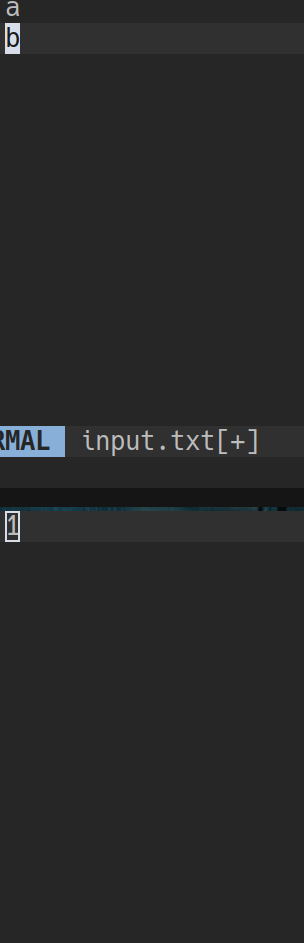
\includegraphics[scale=0.418]{laba0}
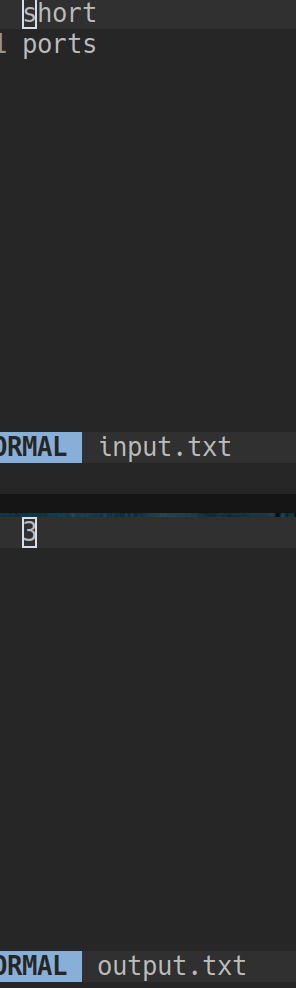
\includegraphics[scale=0.4]{laba1}
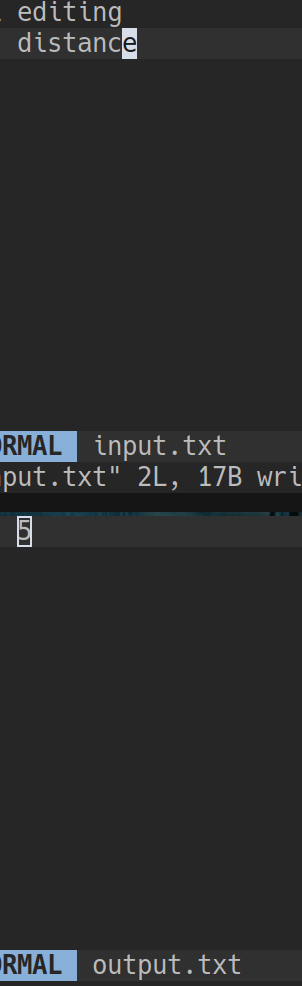
\includegraphics[scale=0.4]{laba2}
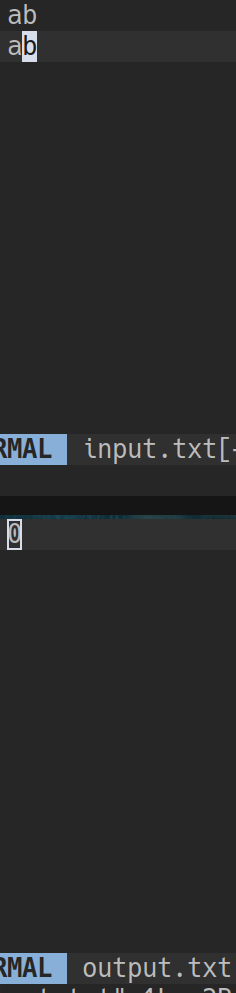
\includegraphics[scale=0.397]{laba3}
\vspace*{1cm}

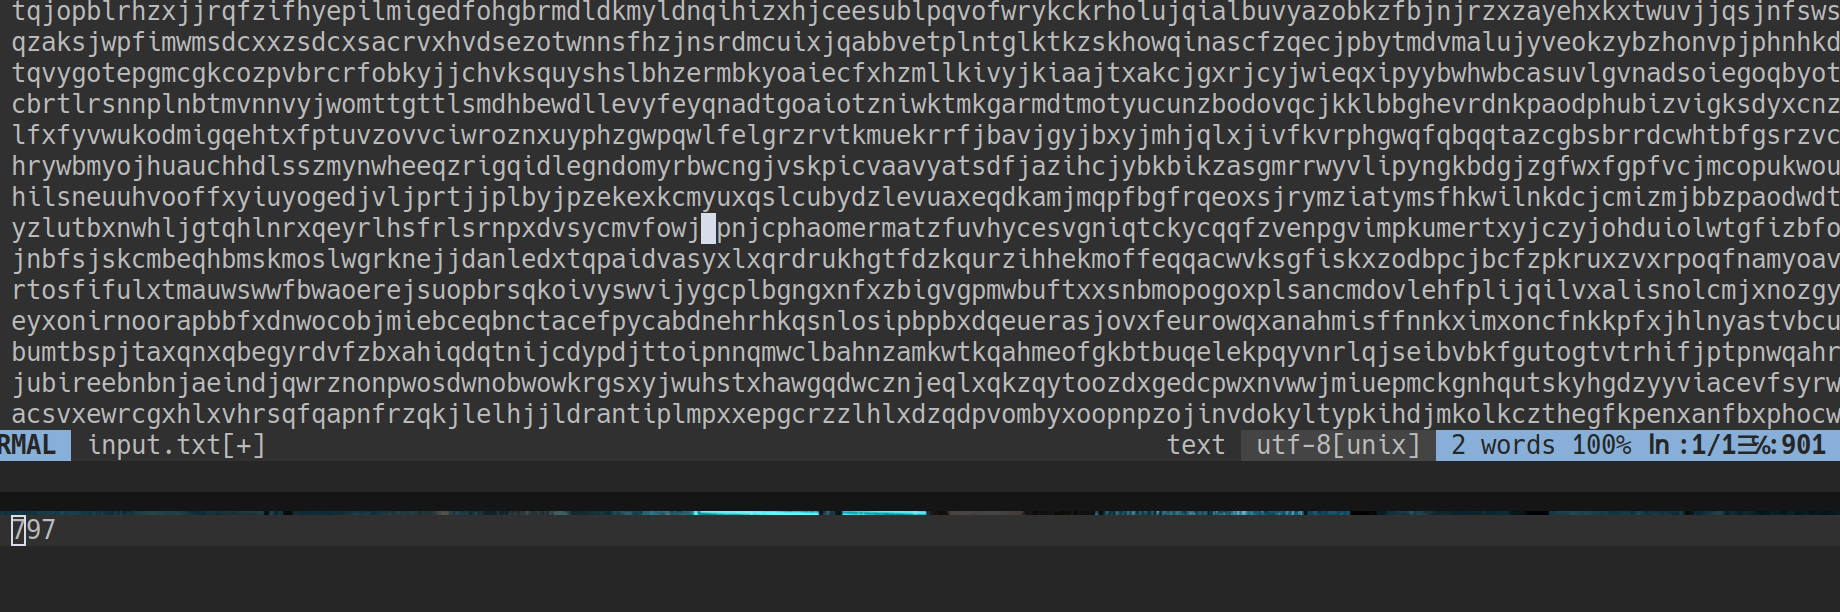
\includegraphics[scale=0.35]{laba4}
\end{center}
\newpage
\begin{tabular}{|p{4cm}|c|c|}
    \hline
     & Время выполнения (с) & Затраты памяти (байт) \\ \hline
    Нижняя граница диапазона значений входных данных из текста задачи & 0.00017152299915323965 & 13939 \\ \hline
    Пример из задачи 1 & 0.0001822340000217082 & 13941 \\ \hline
    Пример из задачи 2 & 0.00019643999985419214 & 13947 \\ \hline
    Пример из задачи 3 & 0.0002520400003049872 & 13952 \\ \hline
    Верхняя граница диапазона значений входных данных из текста задачи & 1.9091916950001178 & 92904 \\ \hline
\end{tabular}
\vspace*{0.5cm}
\newline
\textbf{Вывод по задаче:} Расстояние Левенштайна считается самым эффективным алгоритмом для расчета редакционного расстояния. Его сложность - O(\(n^2\))

\subsection{Задача №4. Наибольшая общая подпоследовательность}
Вычислить длину самой длинной общей подпоследовательности из двух по следовательностей. 
Даны две последовательности A = (a1, a2, ..., an) и B = (b1, b2, ..., bm), найти длину их самой длинной общей подпоследовательности, т.е. наибольшее неотри цатеьное целое число p такое, что существуют индексы 1 ≤ i1 < i2 < ... < ip ≤ n и 1 ≤ j1 < j2 < ... < jp ≤ m такие, что ai1 = bj1, ..., aip = bjp. 

\section{Теоретическая информация}
bash \cite{bash} \\

\section{Ход выполнения работы}

\subsection{Список}

\begin{itemize}
	\item первый элемент списка
	\item второй элемент списка
\end{itemize}


\subsection{Картинка}

\begin{figure}[H]
	\begin{center}
		
\includegraphics[scale=0.7]{sample}
		\caption{название картинки}
		\label{pic:pic_name} % название для ссылок внутри кода
	\end{center}
\end{figure}

Текст без отступа (следует за вставкой)

Новый параграф

\noindent Новый параграф с принудительно выключенным отступом


\subsection{Таблицы}

\begin{table}[H]
	\caption{Одна таблица}
	\begin{center}
		\begin{tabular*}{0.4\textwidth}{@{\extracolsep{\fill} } lcc}
			\toprule
			Element & First & Second \\
			\midrule
			One       & -    & -    \\
			Two       & -    & -    \\
			Three     & -    & -    \\
			Four      & -    & -    \\
			\bottomrule
		\end{tabular*}
		\label{tabular:tab_examp_1}
	\end{center}

	\caption{Другая таблица}
	\begin{center}
		\begin{tabular}{|l|c|r|}
			\hline
			top left & top center & top right \\ \hline
			bot left & bot center & bot right \\ \hline
		\end{tabular}
		\label{tabular:tab_examp_2}
	\end{center}
\end{table}


\newpage
\subsection{Листинг}
\begin{code}
	\inputminted[breaklines=true, xleftmargin=1em, linenos, frame=single, framesep=10pt, fontsize=\footnotesize, firstline=1, lastline=33]{haskell}{listings/script.bash}
	\caption{Script.bash – bash в массы!}
\end{code}

\newpage
\section*{Заключение}
\LaTeX\ удобен для создания отчётов, так как сам следит за нумерацией таблиц, рисунков, листингов и отсылок к ним (так, например, здесь всегда будет указан номер рисунка "sample" не зависимо от того, какой он (1,2 или другой) - это рисунок \ref{pic:pic_name}). Не менее важно что весь документ оформлен в едином стиле, а исходные материалы подключаются к отчёту, а не хранятся в нём. Всё это позволяет легко получить качественный отчёт без дополнительных трат на его офрмление.

Исключения, пожалуй, составляют таблицы, так как их значительно сложнее создавать кодом, нежели в графическом редакторе. Но здесь никто не запрещает использовать визуальные средства создания таблиц для \LaTeX\ .
\addcontentsline{toc}{section}{Заключение}
